\setcounter{section}{1}
\section{Теория множеств}

\subsection{Множество, основные теоретико-множественные операции, декартово произведение}
\begin{itemize}
    \item [] \textit{Множества} состоят из элементов. Запись x $\in$ M означает, что x является элементом множества M.
    \item [] Говорят, что множество A является \textit{подмножеством} множества B (запись: A $\subset$ B), если все элементы A являются элементами B.
    \item [] Множества A и B  \textit{равны} (запись: A = B), если они содержат
одни и те же элементы (другими словами, если A $\subset$ B и B $\subset$ A).
\item [] Если A — подмножество B, не равное всему B, то A называют
 \textit{собственным подмножеством} B

 \item [] Пустое множество $\emptyset$ не содержит ни одного элемента и является подмножеством любого множества.

 \item []   \textit{Пересечение} A $\cap$ B двух множеств A и B состоит из элементов, которые принадлежат обоим множествам A и B. Это записывают так: A  $\cap$ B = $\{x | x \in A$ и $x \in B\}$ 
 \item []  \textit{Объединение} A$\cup$B состоит из элементов, которые принадлежат хотя бы одному из множеств A и B:
A  $\cup$ B = $\{x | x \in A$ или $x \in B\}$ 

 \item []  \textit{Разность} A $\backslash$ B состоит из элементов, которые принадлежат A, но не принадлежат B:
A  $\backslash$ B = $\{x | x \in A$ и $x \not\in B\}$ 

Если множество B является подмножеством множества A, разность A $\backslash$ B называют также дополнением B до A. \\ \\
Симметрическая разность A $\triangle$ B состоит из элементов, которые принадлежат ровно одному из множеств A и B:

 \item [] A $\triangle$ B = (A $\backslash$ B) $\cup$ (B $\backslash$ A) = (A $\cup$ B) $\backslash$ (A $\cap$ B).
\end{itemize}
\begin{center}
    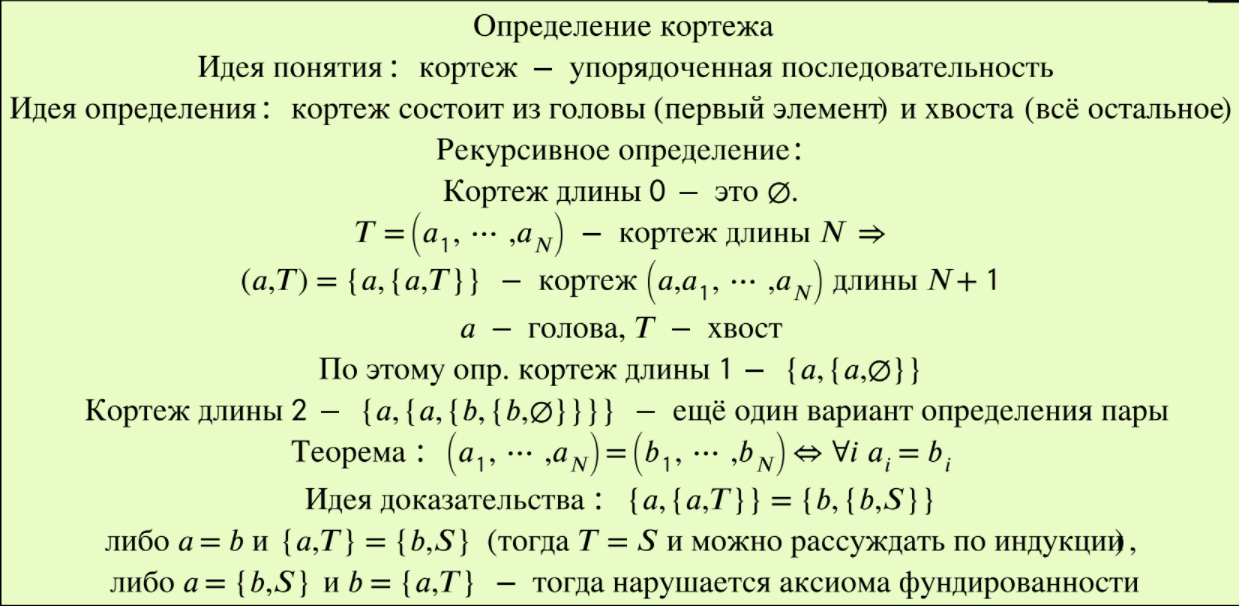
\includegraphics[width = 14cm]{images/2 (определения)_21.PNG}
\end{center}
\textbf{Опр} \textit{Декартово произведение} $A \times B = \{(a,b) | a \in A, b \in B\}$

\subsection{Отображения и соответствия. Образ и прообраз. Инъекции, сюръекции, биекции. Композиция отображений. Возведение множества в степень множества}

\textbf{Опр} \textit{Соответствие} между A и B - это любое множество пар из $A \times B$. Обозначения: $F \subset A \times B, \ F:A\rightarrow B, \ F: A \rightrightarrows B, (a,b) \in F, b \in F(a)$
\\
\textbf{Опр} \textit{Отображение} - это однозначное соответствие, т.е. $\forall \ x \exists!y (x,y) \in F $ 
\\
\textbf{Опр} \textit{Инъективное соответствие}: если $x \neq y$, то $F(x) \cap F(y) = \o$
\\
\textbf{Опр} \textit{Инъекция} - это инъективное отображение: если $x \neq y$, то $F(x) \neq F(y)$
\\
\textbf{Опр} \textit{Сюръективное соответствие}: если $\forall y \exists x \ y \in F(x)$
\\
\textbf{Опр} \textit{Сюръекция} - это сюръективное отображение:  $\forall y \exists x \ y = F(x)$
\\
\\
\textbf{Опр} \textit{Биекция} - это сюръекция + инъекция
\\
Пусть есть соответствие $F: A \rightarrow B, S \subset A, T \subset B$\\
\textbf{Опр} \textit{Образ} S - это множество $F(S) = \cup_{x \in S} F(x) = \{y \ |  \ \exists x \in S \ \ (x,y) \in F\}$
\\
\textbf{Опр} \textit{Проообраз} T - это множество $F^{-1}(T) = \{x \ | \ \exists y\in T \ \ (x,y) \in F\}$
\\
\textbf{Опр} \textit{Композицией отображений} $F : A \rightarrow B, \ G : B \rightarrow C$ называется отображение $H = G \cdot F$, определяемое соотношением $z = H(x) \Longleftrightarrow \ \exists y: y = F(x) $ и $z = G(y)$
\\
\textbf{Опр}
Пусть A и B — два множества. Тогда множеством  $B^A$ называется множество всех отображений из A в B
\\
\subsection{Равномощность. Счётные и континуальные множества.}

\textbf{Опр} Множества А и В назваются \textit{равномщными}, если существует биекция $А \to В$
\\
\textbf{Опр} Множество А называется \textit{счетным}, если оно равномощно множеству $\mathbb{N}$
\\
\textbf{Опр} Множество А называется \textit{континуальным}, если оно равномощно множеству $\mathbb{R}$
\\
\subsection{Бинарные отношения. Отношения эквивалентности и отношения порядка}

\textbf{Опр} \textit{Бинарным отношением на множестве}  A называется любое подмножество $A^2 = A \times A$ или, что тоже
самое, любая функция из $A^2$ в $\{0,1\}$.
\begin{center}
    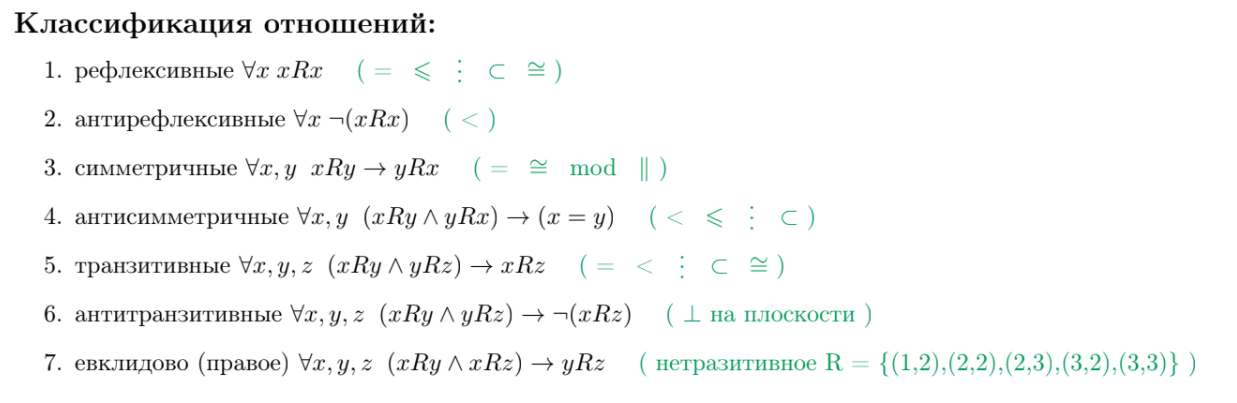
\includegraphics[width = 0.9\textwidth]{images/2 (определения)_m22.PNG}

    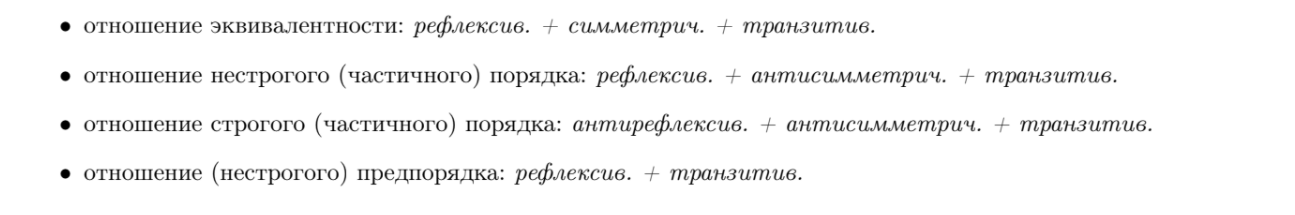
\includegraphics[width = 0.9\textwidth]{images/2 (определения)_m23.PNG}
\end{center}

\subsection{Упорядоченное множество, линейно упорядоченное множество, фундированное множество, вполне упорядоченное множество}

\textbf{Опр} \textit{Упорядоченым множеством}  называется пара $(A, \leq_A)$ - множество и частичный порядок на нем
\\
\textbf{Опр} Частично упорядоченное множество называется \textit{линейно упорядоченным}, если любые два элемента в нем сравнимы
\\
\textbf{Опр} Частично упорядоченное называется \textit{фундированным}, если в любом его непустом подмножестве есть минимальный элемент
\\
\textbf{Пример}
\begin{itemize}
    \item [$\checkmark$] $<\mathbb{N}, \leq>, <\mathbb{N} + \mathbb{N}, \leq>, <\mathbb{N},|>$ с заданным тривиально порядком фундированы
    \item [$\times$] $\mathbb{Z}, [0,1]$ - не фундированы
\end{itemize}
\textbf{Опр} Множество называется \textit{вполне упорядоченным}, если оно линейно упорядочено и фундировано
\\
\textbf{Пример}
\begin{itemize}
    \item [$\times$ ] Множество всех конечных слов из букв латинского алфавита
    \item [$\times$ ] [0,1], $<\mathbb{N},|>$
     \item [$\checkmark$ ] $\mathbb{N}$
\end{itemize}

\subsection{Цепи в упорядоченных множествах. Верхние и нижние грани, максимальные и минимальные, наибольшие и наименьшие элементы}

\textbf{Опр} Подмножество частично упорядоченного множества называется \textit{цепью}, если любые два его элемента сравнимы.
\\
\textbf{Опр} Элемент x $\in$ A \textit{наибольший} в упорядоченном множестве $(A, \leq_A)$, если $\forall y \in A : y \leq_A x$. Элемент x $\in$ A
\textit{максимальный} в упорядоченном множестве $(A, \leq_A)$, если $\not\exists y \in A : x \leq_A y$. Наименьший и минимальный
элементы определяются аналогично.
\\
\textbf{Опр}  \textit{Верхней гранью} множества А называется такой элемент M, что $\forall x \in A \ x\leq M$
\\
\textbf{Опр}  \textit{Нижней гранью} множества А называется такой элемент m, что $\forall x \in A \ x\geq m$
\\
\subsection{Гомоморфизмы и изоморфизмы упорядоченных множеств}

\textbf{Опр} \textit{Гомоморфизмом упорядоченных множеств} называется функция $f:A\rightarrow B$, такая что
\begin{center}
    $x \leq_A y \Longleftrightarrow f(x) \leq_B f(y)$
\end{center}

\textbf{Опр} \textit{Изоморфизмомом  упорядоченных множеств} называется  функция $f:A\rightarrow B$, являющаяся гомоморфизмом и биекцией.

\subsection{Сложение и умножение упорядоченных множеств}


\includegraphics[width = 0.8\textwidth]{images/2 (определения)_m24.PNG}


\includegraphics[width = 0.8\textwidth]{images/2 (определения)_m25.PNG}

\subsection{Начальные отрезки вполне упорядоченных множеств.}
\textbf{Опр} Начальным отрезком ВУМ называется такое $B \subset A$, что $\forall x \in B, \ \forall y \in A \backslash B \ x \leq y$
\\
\textbf{Примеры}
\begin{itemize}
    \item [$\checkmark$] [0,а] = $\{x \ | \ x\leq a\}$
     \item [$\checkmark$][0,а) = $\{x \ | \ x<a\}$
      \item [$\checkmark$] Всё А
\end{itemize}
Если $x \in [0,a] \Longrightarrow \ x\leq a, \ y \in \overline{[0,a]} \Longrightarrow y > a \Longrightarrow x \leq a < y$, откуда x < y. \\
Если множество вполне упорядочено и при этом не пусто. то всем есть наименьший элемент, тогда этот элемент обозначается 0
\\
\subsection{Предельные элементы вполне упорядоченных множеств}

\textbf{Опр} В любом ВУМ у любого элемента, кроме максимального, есть единственный и непосредственно следующий за ним, т.е. такой с > а, что ни для какого b неверно с > b > a (элемент а + 1)
\\
\textbf{Опр} \textit{Предельным элементом ВУМ} называется элемент, не являющийся непосредственно следующим ни за каким другим
\\
\subsection{Порядковые типы $\omega, \omega^k, \omega^{\omega}, \epsilon_0$}
\begin{center}
        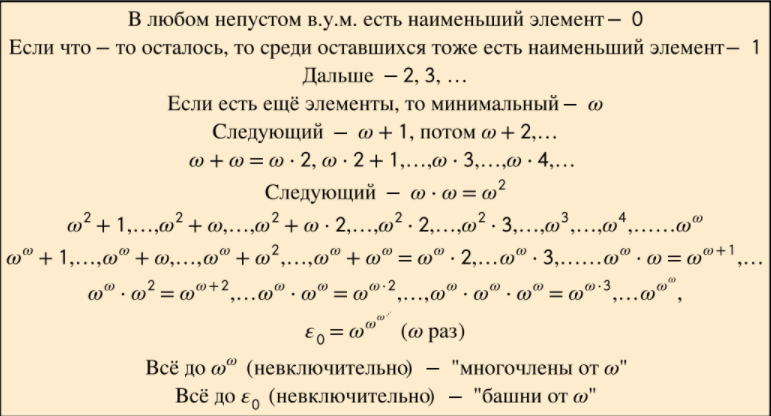
\includegraphics[width = 0.75\textwidth]{images/2 (определения)_m26.PNG}
    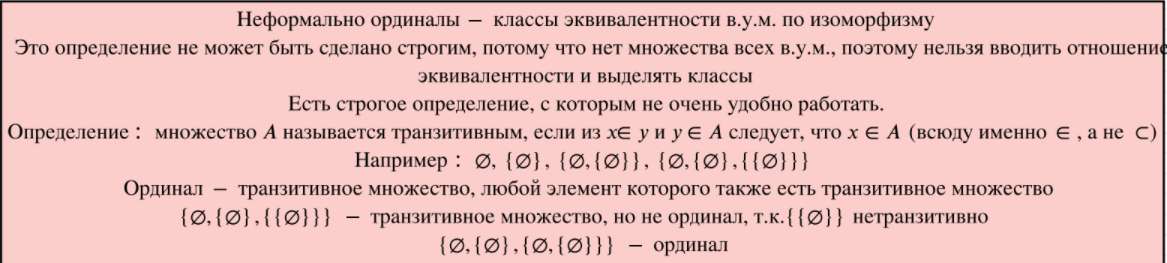
\includegraphics[width = 0.75\textwidth]{images/2 (определения)_m27.PNG}
\end{center}

\subsection{Аксиома выбора}

Пусть задано некоторое множество А. Тогда существует функция $\phi: (2^A\ \backslash \{A\}) \rightarrow A$, такая что $\forall S \ \phi(S) \in A\backslash S$
\\
\subsection{Базис Гамеля}

Базис Гамеля в $\mathbb R$ над $\Q$ это такой набор действительных чисел, что любое другое действительное число представляется как конечная ЛК элементов базиса с рациональными коэффициентами, при этом никакая нетривиальная конечная линейная комбинация элементов базиса с рациональными коэффициентами не равна $0$.